\begin{frame}{Le transistor comme interrupteur commandé}
  \begin{columns}
    \begin{column}{0.5\textwidth}
      \textbf{Transistor NMOS}
      \begin{itemize}
        \item Conduit (interrupteur fermé) si \textbf{Grille = 1}
        \item Bloqué si Grille = 0
        \item \fbox{Transmet bien un \textbf{0} logique}
      \end{itemize}
      \vspace{0.5cm}
      \textbf{Transistor PMOS}
      \begin{itemize}
        \item Conduit (interrupteur fermé) si \textbf{Grille = 0}
        \item Bloqué si Grille = 1
        \item \fbox{Transmet bien un \textbf{1} logique}
      \end{itemize}
    \end{column}
    \begin{column}{0.5\textwidth}
      \centering
      \begin{circuitikz}[scale=1.0]
        \draw (0,0) node[nmos, anchor=D](M1){};
        \draw (M1.G) node[left=0.3cm]{$G$};
        \draw (M1.S) node[below=0.2cm]{$S$};
        \draw (M1.D) node[above=0.2cm]{$D$};
      \end{circuitikz}
      \hspace{0.5cm}
      \begin{circuitikz}[scale=1.0]
        \draw (0,0) node[pmos, anchor=D](M2){};
        \draw (M2.G) node[left=0.3cm]{$G$};
        \draw (M2.S) node[above=0.2cm]{$S$};
        \draw (M2.D) node[below=0.2cm]{$D$};
      \end{circuitikz}
    \end{column}
  \end{columns}
\end{frame}
%
\begin{frame}{Table de fonctionnement simplifiée}
  \centering
  \begin{tabular}{ccc}
    \toprule
    Entrée grille & NMOS & PMOS \\
    \midrule
    0 & bloqué & passant \\
    1 & passant & bloqué \\
    \bottomrule
  \end{tabular}
  \vspace{0.5cm}

  \begin{block}{Idée fondatrice du CMOS}
    On associe systématiquement un réseau de NMOS (relié à la masse)
    et un réseau de PMOS \emph{dual} (relié à l'alimentation $V_{DD}$)
    pour qu'à chaque instant \textbf{un seul} des deux réseaux conduise.
  \end{block}
\end{frame}
%
% ------------------------------------------------------------
%\section{L'inverseur CMOS}

\begin{frame}{L'inverseur CMOS : la porte de base}
  \begin{columns}
    \begin{column}{0.35\textwidth}
      \begin{circuitikz}[scale=1.1, transform shape]
        % --- Alimentation ---
        \draw (0,4.6) node[above]{$V_{DD}$};
        \draw (0,4.6) to[short] (0,4.1);
        % --- PMOS ---
        \draw (0,4.1) node[pmos, anchor=S](P1){};
        % --- Noeud de sortie Y ---
        \draw (P1.D) to[short] (0,2.6);
        \draw (0,2.6) to[short] (0.7,2.6) node[right]{$Y$};
        % --- NMOS ---
        \draw (0,2.6) node[nmos, anchor=D](N1){};
        % --- Connexion des grilles ---
        \draw (P1.G) -- ++(-0.8,0) coordinate(pgate);
        \draw (N1.G) -- ++(-0.8,0) coordinate(ngate);
        \draw (pgate) -- (ngate);
        % --- Entrée A alignée avec Y ---
        \coordinate (aPoint) at (pgate |- N1.D);
        \draw (aPoint) -- ++(-0.5,0) node[left]{$A$};
        % --- Masse ---
        \draw (N1.S) to[short] (0,1.1);
        \draw (0,1.1) node[ground]{};
      \end{circuitikz}
    \end{column}
    \begin{column}{0.65\textwidth}
      \begin{itemize}
        \item Entrée $A$ commune aux deux grilles
        \item PMOS en haut (côté $V_{DD}$)
        \item NMOS en bas (côté masse)
        \item Si $A=0$ : PMOS passant, NMOS bloqué $\Rightarrow Y=1$
        \item Si $A=1$ : PMOS bloqué, NMOS passant $\Rightarrow Y=0$
      \end{itemize}
      \vspace{0.3cm}
      \[ Y = \overline{A} \]
    \end{column}
  \end{columns}
\end{frame}

\begin{frame}{L'inverseur CMOS : chronogramme}
  \begin{center}
    %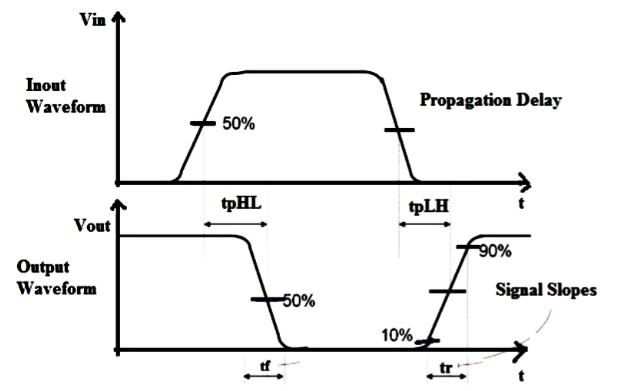
\includegraphics[scale=0.5]{./images/inverter_slopes.png}
    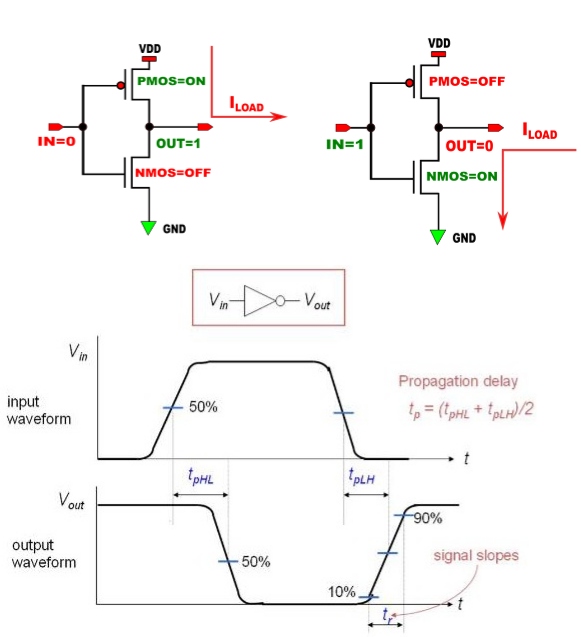
\includegraphics[scale=0.45]{./images/inverter.png}
  \end{center}
\end{frame}

\begin{frame}{Porte NAND à 2 entrées : montage dual}
  \begin{columns}
    \begin{column}{0.35\textwidth}
      \begin{circuitikz}[scale=1.0, transform shape]
        % --- Rail VDD ---
        \draw (-1.6,6.0) node[above]{$V_{DD}$} to[short] (2.2,6.0);

        % --- PMOS A (gauche) ---
        \draw (-0.8,6.0) to[short] (-0.8,5.6);
        \node[pmos, anchor=S] (Pa) at (-0.8,5.6) {};
        \draw (Pa.G) -- ++(-0.3,0) node[left]{$A$};

        % --- PMOS B (droite) ---
        \draw (1.4,6.0) to[short] (1.4,5.6);
        \node[pmos, anchor=S] (Pb) at (1.4,5.6) {};
        \draw (Pb.G) -- ++(-0.3,0) node[left]{$B$};

        % --- Jonction des deux drains PMOS (en parallele) ---
        \draw (Pa.D) -- (-0.8,4.3) -- (0.3,4.3);
        \draw (Pb.D) -- (1.4,4.3) -- (0.3,4.3);
        \draw (0.3,4.3) -- (0.3,3.6);

        % --- Noeud de sortie Y, sorti sur le cote pour eviter le chevauchement ---
        \draw (0.3,3.6) to[short] (1.6,3.6) node[right]{$Y$};
        \filldraw (0.3,3.6) circle (0.05);

        % --- NMOS A (haut de la pile) ---
        \node[nmos, anchor=D] (Na) at (0.3,3.6) {};
        \draw (Na.G) -- ++(-0.9,0) node[left]{$A$};

        % --- NMOS B (bas de la pile), en serie avec Na ---
        \node[nmos, anchor=D] (Nb) at (0.3,2.3) {};
        \draw (Na.S) -- (Nb.D);
        \draw (Nb.G) -- ++(-0.9,0) node[left]{$B$};

        % --- Masse ---
        \draw (Nb.S) -- (0.3,1.0) node[ground]{};
      \end{circuitikz}
    \end{column}
    \begin{column}{0.65\textwidth}
      \begin{itemize}
        \item NMOS $A$ et $B$ en \textbf{série} $\to$ conduit
          seulement si $A=1$ ET $B=1$
        \item PMOS $A$ et $B$ en \textbf{parallèle} (dual)
        \item $Y=0$ uniquement si $A=B=1$
      \end{itemize}
      \[ Y = \overline{A \cdot B} \]
    \end{column}
  \end{columns}
\end{frame}

\begin{frame}{Pourquoi ça marche : jamais de court-circuit}
  \begin{itemize}
    \item En régime statique, un seul chemin conducteur existe entre
      $V_{DD}$ et $Y$, ou entre $Y$ et la masse — jamais les deux.
    \item Conséquence : \textbf{pas de consommation statique}
      (hors fuites), contrairement aux logiques NMOS seules
      (résistance de charge) ou bipolaires.
    \item La consommation du CMOS est essentiellement
      \textbf{dynamique} : elle a lieu lors des commutations
      (charge/décharge des capacités de sortie).
  \end{itemize}
\end{frame}

\begin{frame}{Dualité N-P en CMOS : autre exemple}
  \begin{center}
    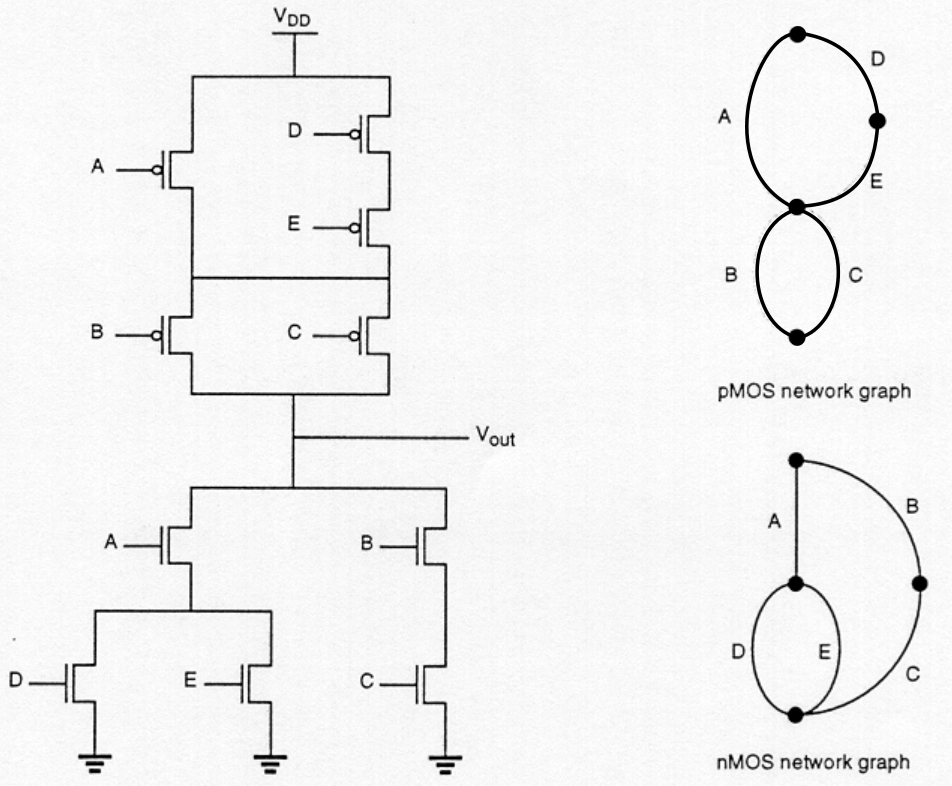
\includegraphics[scale=0.35]{./images/dualite_eulerien.png}
  \end{center}
\end{frame}

% % ------------------------------------------------------------
% \section{Porte NAND}
%
% \begin{frame}{Porte NAND à 2 entrées}
%   \begin{columns}
%     \begin{column}{0.55\textwidth}
%       \begin{circuitikz}[scale=1.0, transform shape]
%         % --- Rail VDD ---
%         \draw (-0.8,5.2) node[above]{$V_{DD}$};
%         \draw (-0.8,5.2) to[short] (1.4,5.2);
%         % --- PMOS A (gauche) et PMOS B (droite), en parallele ---
%         \draw (-0.8,5.2) to[short] (-0.8,4.7);
%         \draw (-0.8,4.7) node[pmos, anchor=S](Pa){};
%         \draw (Pa.G) -- ++(-0.8,0) node[left]{$A$};
%         \draw (1.4,5.2) to[short] (1.4,4.7);
%         \draw (1.4,4.7) node[pmos, anchor=S](Pb){};
%         \draw (Pb.G) -- ++(0.8,0) node[right]{$B$};
%         % --- jonction des deux drains PMOS vers Y ---
%         \draw (Pa.D) to[short] (-0.8,3.8) to[short] (0.3,3.8);
%         \draw (Pb.D) to[short] (1.4,3.8) to[short] (0.3,3.8);
%         \draw (0.3,3.8) to[short] (0.3,3.2);
%         \draw (1.1,3.2) node{$Y$};
%         % --- NMOS A et B en serie ---
%         \draw (0.3,3.2) node[nmos, anchor=D](Na){};
%         \draw (Na.G) -- ++(-0.8,0) node[left]{$A$};
%         \draw (Na.S) to[short] (0.3,1.9);
%         \draw (0.3,1.9) node[nmos, anchor=D](Nb){};
%         \draw (Nb.G) -- ++(-0.8,0) node[left]{$B$};
%         \draw (Nb.S) to[short] (0.3,0.9);
%         \draw (0.3,0.9) node[ground]{};
%       \end{circuitikz}
%     \end{column}
%     \begin{column}{0.45\textwidth}
%       \begin{itemize}
%         \item NMOS $A$ et $B$ en \textbf{série} $\to$ conduit
%           seulement si $A=1$ ET $B=1$
%         \item PMOS $A$ et $B$ en \textbf{parallèle} (dual)
%         \item $Y=0$ uniquement si $A=B=1$
%       \end{itemize}
%       \[ Y = \overline{A \cdot B} \]
%     \end{column}
%   \end{columns}
% \end{frame}
